\documentclass{article}
\usepackage{amsmath,amssymb,amsthm,enumitem} % Some standard math packages.
\usepackage{titling} % Enables \setlength{\droptitle}
\usepackage{parskip} % Cleaner paragraph display
\usepackage[margin=1in]{geometry} % Adjusts margins.
\usepackage[utf8]{inputenc} % USe UTF-8 input encoding instead of default ASCII.
\usepackage[]{forest} % Draws trees.
\usepackage{fancyvrb} % Allows Verbatim sections with line numbers and such. Note the capital V.
\usepackage{pgfplots}
\pgfplotsset{compat=1.6}
\newcommand {\todo}[1] {{\textbf{\color{red}#1}}}

\title{CS 584 Research Project}
\author{ Dylan Laufenberg }
\date{June 5, 2018}

\begin{document}
\maketitle

\paragraph{Project topic} I will implement a variety of data structures that maintain total orders on their data, e.g. 2-3 trees, treaps, and skip lists; I will choose at least one deterministic structure as a reference and at least one randomized data structure for comparison. I will experimentally evaluate the rates of growth of their run times for insertions, searches, and deletions. Based on these data, I will discuss how the performance I observe compares to the predicted asymptotic performance.

\section{Introduction}
This paper aims to illuminate various facets of the relationship between asymptotic complexity and empirical performance of a range of related data structures. The vehicle for this exploration is a series of benchmarks of data structures that perform similar jobs in very different ways. These include binary search trees, treaps, and skip lists \todo{FINALIZE LIST OF DATA STRUCTURES}. For many tasks, they have the same asymptotic complexity, e.g. average complexity of $O(\log n)$ for search, insert, and delete operations, with worst-case complexity of $O(n)$ for each. This paper examines the performance characteristics of each and investigates how comparable the performance characteristics of these asymptotically equivalent data structures really are.

\section{Testing Methodology}

The core of the analysis in this paper is a collection of data sets gathered through benchmarking. Thus, it is essential to establish a reliable testing methodology, enforced through automation, to gather accurate data and ensure the integrity of the analysis that follows. The benchmarking procedure is standardized and automated through benchmark.py.

Noise in the graphs is of paramount importance to the accuracy of the data sets. To smooth out small spikes in running times, each data point in each test consists of 1,000 operations. (This also reduces the impact of the error inherent in the timer.) At the start of the operation, the data structure contains the number of elements indicated on the graph. For instance, a data point for the insertion operation and labeled as having a data structure size of 100,000 elements consists of the average running time for the insertion operations on elements 100,001 through 101,000. This, of course, affects the overall result, as the final element is likely to require more work than the first element (in the case of insertion). In order to minimize these differences, the data structure sizes are no smaller than 100,000 elements, so that the greatest variation in data structure size from the start of any given data point's sample range to the end of the range is 1\%.

In order to compensate for larger variations in system load and running time, each benchmark as described above is run three times on the same input data, and for each data point, the median of the three runs is used.

Having addressed the major issues of unpredictable CPU-time fluctuations, a problem of predictable CPU-time fluctuations remains: the type of test data chosen can affect the integrity of the tests themselves. Strings as keys, of course, are poor choices, since they take linear time to compare (at least using simple string comparison). Objects with numeric keys might simulate real-world conditions well (as might strings), but they, too, may add a degree of instability to the test results, even given that Python passes references to objects. The simplest choice, with the highest likelihood of consistent performance, seems to be simple integers (within the limit of an architecture's word size). Near-constant-time integer comparisons and assignments should minimize the data themselves as sources of noise in the benchmarks to follow.

\todo{Shorten the above paragraphs}

\section{Project Files}
The Python 3 implementations included with this report are structured as follows:
\begin{itemize}
    \item datastructures/ --- contains the implementations of data structures benchmarked below, one per file.
    \item plots/ --- contains the output \LaTeX \ figures that the benchmark system produces, ready to \\include.
    \item pgfplot.py --- contains the PgfPlot class, which represents one \LaTeX \ figure to be produced. This class receives and stores all parameters that affect the figure, including plots to be produced.
    \item plot.py --- contains the Plot and BenchmarkPlot classes, which represent plots in a PGFPLOT graph. The Plot class may be used to produce arbitrary plots, whereas the BenchmarkPlot class receives benchmark parameters for one function and produces the corresponding plot.
    \item benchmark.py --- sets up and runs the benchmarks used in this document by creating PgfPlot objects and running them.
\end{itemize}

To run custom benchmarks, simply follow the examples in benchmark.py. All classes are thoroughly documented and commented.

\section{Data Structure Selection}
Many implementations exist for each of these data structures, since they are well-known. 

\todo{Charts here comparing different implementations of various data structures}

\newpage
\section{Testing TikZ Pictures}

\begin{figure}[h]
    \centering
    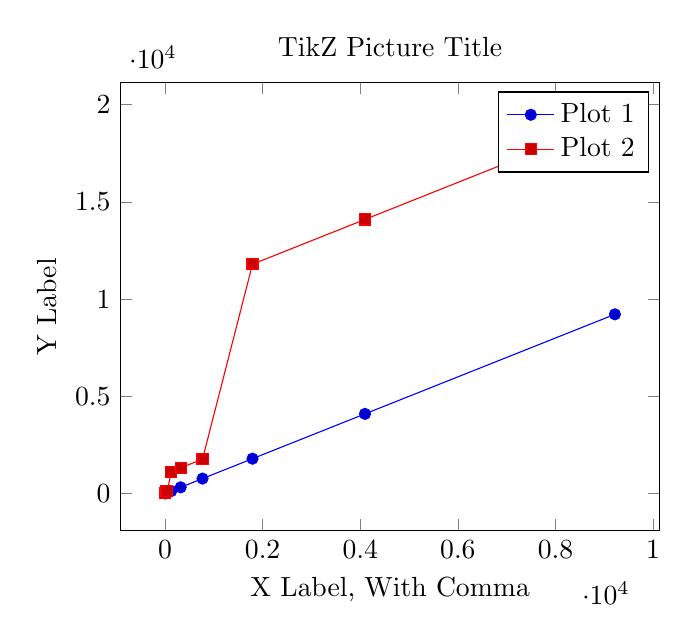
\begin{tikzpicture}
        \begin{axis}[xlabel={
            X Label, With Comma}, 
            ylabel=Y Label, 
            title=TikZ Picture Title
        ]
        \addplot coordinates {
            (5, 6)
            (17, 18)
            (49, 50)
            (129, 130)
            (321, 322)
            (769, 770)
            (1793, 1794)
            (4097, 4098)
            (9217, 9218)
        };
        \addplot coordinates {
            (5, 16)
            (17, 118)
            (49, 150)
            (129, 1130)
            (321, 1322)
            (769, 1770)
            (1793, 11794)
            (4097, 14098)
            (9217, 19218)
        };
        \legend{Plot 1, Plot 2}
        \end{axis}
    \end{tikzpicture}
    \caption{Figure Caption}
\end{figure}

\begin{figure}[h]
    \centering
    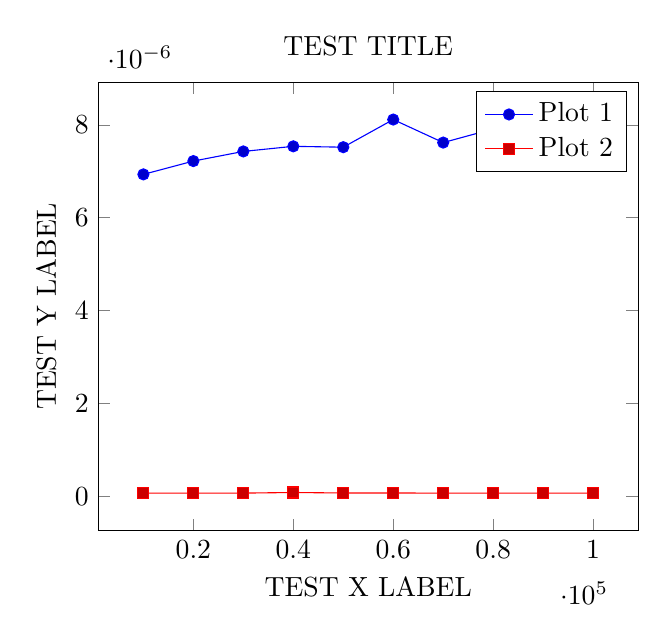
\begin{tikzpicture}
        \begin{axis}[
            xlabel={TEST X LABEL},
            ylabel={TEST Y LABEL},
            title={TEST TITLE}
        ]
		\addplot coordinates {
			(10000, 6.933658602697013e-06)
			(20000, 7.219775172611076e-06)
			(30000, 7.427586154969745e-06)
			(40000, 7.537515152884033e-06)
			(50000, 7.5188422820053894e-06)
			(60000, 8.11396474742665e-06)
			(70000, 7.618230143133564e-06)
			(80000, 7.911574921129593e-06)
			(90000, 7.978737021225424e-06)
			(100000, 7.994096963399588e-06)
		};
		\addplot coordinates {
			(10000, 7.167973014698959e-08)
			(20000, 7.167973014698959e-08)
			(30000, 7.198090548321545e-08)
			(40000, 8.523262030069035e-08)
			(50000, 7.408913284079333e-08)
			(60000, 7.439030817746329e-08)
			(70000, 7.137855480987553e-08)
			(80000, 7.137855481031963e-08)
			(90000, 7.137855480987553e-08)
			(100000, 7.107737947364967e-08)
		};
        \legend{Plot 1, Plot 2}
        \end{axis}
    \end{tikzpicture}
    \caption{TEST CAPTION}
\end{figure}

\end{document}
